\chapter{Self-Directed Experiment}

You've spent the last 4 weeks learning various techniques for collecting and analyzing astronomical data. Now it's your turn to choose a project and use those techniques more independently to answer a scientific question that you choose. At least, you can choose from a list, so it is more likely you'll find a project that appeals to you.

So in the next two weeks, you will conduct the experiment / project, and in the following week, you will present your findings in class (as well as submitting a written report). Our goal is for you to work more independently than in past weeks, and also use your TA, professor, and teaching support manager for assistance when needed.

\section{Picking a Project}

\begin{steps}
	\item Individually, read through the available projects and pick your favorite, writing it on the board.
	
	\item Once everyone has written their preference, if any project has more than the max number of people listed for the project, people will be chosen at random to be in that project.
	
	\item The remaining people without projects pick from the understaffed projects that remain and the random selection happens again, until all students have a project, and each project has the minimum group size.
\end{steps}

%\section{Project A: Pillars of Creation}
%
%For nearly the last three decades, Hubble Space Telescope has been pointed towards the heavens, taking images of space. Take a look at the images in Figure\ \ref{sp:fig:pillars}, taken by the Hubble Space Telescope. While both images are of the same subject matter, they look completely different, why is that? Demonstrate quantitatively using some sample values why these two appear different. Write up a little bit about what you see here in these images, how you know what you are looking at, and why it is interesting to astronomers.
%
%\begin{figure}
%	\centering
%	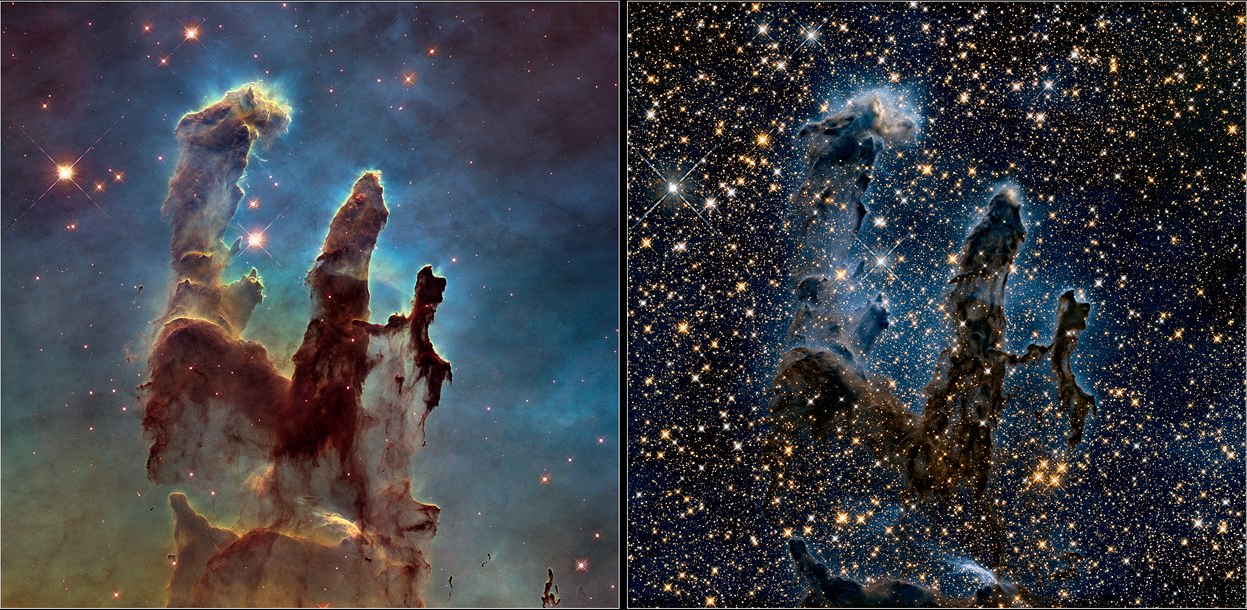
\includegraphics[width=\textwidth]{stars-project/heic1501c-crop}
%	\caption{Two images of the same part of the sky.}\label{sp:fig:pillars}
%\end{figure}

\section{Project A: When did the Crab Nebula star explode?}

\textbf{Group size:} 2

The Crab Nebula (M1) is a supernova remnant that has been observed by humans for nearly 1000 years. The force of the supernova propels gas outward, expanding into space. But just how fast is it expanding? Calculate the velocity (with uncertainties) of the expansion of the Crab Nebula in km/s. Work backwards and calculate when the Crab Nebula originally exploded, giving your uncertainty for that year.

\textbf{Materials:} archival Crab Nebula images (SEO + \url{https://archive.stsci.edu/cgi-bin/dss_form})

\begin{itemize}
	\item The date an image was taken is found in the header of FITS files. This can be viewed by loading the image in DS9 and selecting File $>$ Display Header...
\end{itemize}

\section{Project B: How heavy is the binary star system 61 Cygni AB?}
\textbf{Group size:} 2

Binary stars afford us an opportunity to determine the mass of the star system using Kepler's laws, since we can view the star's movements over time and calculate orbits. Your mission is to use historical measurements in Table\ \ref{61cyg_data}, and add your own using SEO, to determine the mass of the 61 Cygni AB binary star system.

\begin{itemize}
	\item For two bodies of mass $M_A$ and $M_B$ that are orbiting each other, the period $P$ of the orbit and the semi-major axis of the ellipse swept out by the difference in the positions between bodies A and B., $a$, are related by Newton's version of Kepler's third law,
	\begin{equation}
	P^2 = \frac{4\pi^2}{G(M_A + M_B)}a^3 \,,
	\end{equation}
	where $G$ is the Newtonian constant of gravitation.

	\item To add your values to the historical table, you will need to convert your RA ($\alpha$) and Dec ($\delta$) to separation angle $r$ and position angle $\theta$. You can use the following formulas,
	
	\begin{equation}
	r = \sqrt{[\cos(\delta_{\textrm{avg}}) \: \Delta\alpha]^2 + (\Delta\delta)^2}
	\end{equation}
	and
	\begin{equation}
	\theta = \arctan{\frac{\cos(\delta_{\textrm{avg}})\:\Delta\alpha}{\Delta\delta}}\,,
	\end{equation}
	where $\delta_{\textrm{avg}}$ is the average declination expressed in degrees, $\Delta\alpha$ is the difference in RA of the two stars in arcseconds, and $\Delta\delta$ is the Dec difference in arcseconds. The difference should always be the fainter star minus the brighter star.
	
	\item To get the orbital parameters $P$ and $a$, you'll probably want to plot the ellipse visually and estimate from there. To do that easily, you may want to convert the data from polar coordinates $(r,\theta)$ to rectangular $(x,y)$ values. See \url{https://www.mathsisfun.com/polar-cartesian-coordinates.html} for assistance with this. You can use these formulas:
	\begin{equation}
	x = r\cos\theta\;\;\;y = r\sin\theta
	\end{equation}
	To put $x$ and $y$ in physical units, divide these values by the measured parallax of the system, 0.314 arcsec, which gives the distances in AU.
	
	\item Report your result in both kilograms and number of solar masses. Include estimation of uncertainty.
\end{itemize}

\begin{table}
	\centering
	\caption{Historical Data for 61 Cyg AB}
	\label{61cyg_data}
	\begin{tabular}{|l|c|c|r|}
		\hline
		\textbf{Date} & \textbf{Separation $r$ (arcsec)} & \textbf{Position Angle $\theta$ (\textdegree)} & \textbf{Reference} \\
		\hline
		1753 & 19.6 & 35 & J. Bradley, obtained via WVDSC\\
		1838 & 16.204 & 95.325 & Bessel 1938, AN, 16, 65\\
		1914 & 23.3 $\pm$ 1.4 & 136.4 $\pm$ 3.5 & Yerkes Plates\\
		1951 & 26.3 $\pm$ 3.0 & 141 $\pm$ 7 & Digitized Sky Survey, Blue I\\
		2019 & & & your measurement\\
		\hline
	\end{tabular}
\end{table}

\section{Project C: What elements are in the Sun?}

\textbf{Group size:} 2--3

Determine what elements in the atmosphere of the Sun by comparing the spectrum of the Sun to the spectrum of light given off by those elements when they have high voltage applied to them. First, familiarize yourself with analyzing spectra by using gas discharge tubes and the digital spectrometer in the lab and identifying unknown elements (a list of prominent wavelengths is found in Table\ \ref{sp:tab:emissions}). Then, sign up with Prof.\ Fabrycky to use the telescope on the roof of Kersten to take a spectrograph of the Sun and identify hydrogen and sodium by comparing to the spectra taken with gas discharge lamps. Finally, identify at least two other elements by comparing your spectra to the spectral atlas found at \url{http://bass2000.obspm.fr/download/solar_spect.pdf}.

\begin{table}
	\centering
	\begin{tabular}{c|c|c|c}
		\toprule
		\textbf{Helium (nm)} & \textbf{Argon (nm)} & \textbf{Neon (nm)} & \textbf{Mercury (nm)} \\ \midrule
		389 & 697 & 585 & 365 \\
		447 & 707 & 594 & 404 \\
		469 & 738 & 614 & 435 \\
		492 & 751 & 627 & 546 \\
		502 & 764 & 640 & 579 \\
		588 & 772 & 651 & \\
		668 & 795 & 660 & \\
		707 & 801 & 668 & \\
		727 & 811 & 693 & \\
		& 826 & 703 & \\
		& 841 & 717 & \\
		& 852 & 744 & \\
		& 866 & & \\
		& 912 & & \\ \bottomrule
	\end{tabular}
	\caption{Some known emission lines of various elements.}\label{sp:tab:emissions}
\end{table}

\begin{itemize}
	\item You must be available to take data with Prof.\ Fabrycky using the Dunham telescope, during one of these two windows of time: Nov 12 9:00a--12:00p; Nov 14 1:00--4:00p. Email him to arrange when to meet during that time.
\end{itemize}

\section{Project D: How fast are stars moving?}

\textbf{Group size:} 2

Humans have been looking at the sky for thousands of years, and the sky is ever changing. Here is a tinyyy fraction (a few decades) worth of archival imagery for you to peruse (\url{https://archive.stsci.edu/cgi-bin/dss_form}). Select your favorite patch of the sky, and see how it changes over time. In particular, find a star that moves significantly over the course of these decades, and tell us just how quickly this star is moving in angular velocity (for example, in milliarcseconds/year). Check your answer using Stellarium. Use Stellarium to find the distance to this star and convert the angular speed to a physical speed in m/s. Compare this to human-scale speeds to gain perspective (e.g.\ a running human, plane, Elon Musk's Hyperloop).

\begin{itemize}
	\item Do this for 4 stars and include uncertainty estimates for your speeds.
\end{itemize}

\begin{itemize}
	\item The date an image was taken is found in the header of FITS files. This can be viewed by loading the image in DS9 and selecting File $>$ Display Header...
	
	\item To compare two images of the same part of the sky, you can open both in DS9 and ``blink'' between them. To do so, first open one image normally. Then select Frame $>$ New Frame, and then use File $>$ Open... to open the second image. Next, align the two images together by selecting Frame $>$ Match $>$ Frame $>$ WCS. Then you can blink between them with Frame $>$ Blink Frames.
\end{itemize}

\section{Project E: Fun with GAIA}

\textbf{Group size:} 3

GAIA is an ongoing mission that measures stellar proper motion --- the motion of the star perpendicular to the observer’s line of sight. We’ve downloaded some data for you to play with in Excel (or programming language of your choice). Please make the following plots and answer the associated questions. Be very specific, even though the questions seem quite general:

\begin{enumerate}
	\item \textbf{RA vs. Dec.} What structure do you see, if any?
	
	\item \textbf{Color vs. Temperature.} What does this trend tell you?
	
	\item \textbf{Luminosity vs. Temperature (aka H-R Diagram).} Make sure the axes are scaled properly and go the standard direction for H-R diagrams.
	
	\item \textbf{Luminosity vs. Color.} Why does this look better than the typical HR diagram in the last plot?
	
	\item \textbf{Color vs. Parallax.} What is the structure? Describe what you see and why things look that way.
\end{enumerate}

\subsection{Notes}

\begin{itemize}
	\item The description of the headers of the file can be found here: \url{https://gea.esac.esa.int/archive/documentation/GDR2/Gaia_archive/chap_datamodel/sec_dm_main_tables/ssec_dm_gaia_source.html}
	
	\item The various filter passbands (what wavelengths the filter lets through) can be seen here: \url{https://www.cosmos.esa.int/web/gaia/iow_20180316}
\end{itemize}

\section{Report checklist and grading}

Each group will submit one (1) report for the group. The report must list specifically how each group member contributed to the report.

Each item below is worth 10 points, and there is an additional 10 points for attendance and participation. See Appendix\ \ref{cha:lab-report-format} for guidance on writing the report and formatting tables and graphs.

\begin{enumerate}
	\item To be determined.
\end{enumerate}

\section{Presentation parameters}

Each group will give a 10 minute presentation, with a question period following. Students are encouraged to ask questions of each other. During the questions, the TA will ask each group member a question that they need to answer themselves, that should be answerable if they know everything that went into the report. The presentation grade will include both a group portion and an individual portion, with the individual portion based on the accuracy of that group member's answer.